\documentclass[16pt]{beamer}
\usetheme[outer/progressbar=foot]{metropolis}
% \usecolortheme{owl}


\definecolor{Purple}{HTML}{911146}
\definecolor{Orange}{HTML}{FF9900}
\definecolor{LightBlue}{HTML}{B3FFFF}
\definecolor{White}{HTML}{FFFFFF}
\definecolor{Black}{HTML}{000000}
\definecolor{Gray}{HTML}{F2F2F2}
% \setbeamercolor{alerted text}{fg=Orange}
\setbeamercolor{frametitle}{bg=Orange,fg=Black}

\setbeamercolor{background canvas}{bg=White}
\setbeamercolor{block title}{bg=Orange,fg=Black}
\setbeamercolor{block body}{bg=Gray,fg=Black}

\usepackage{graphicx}
\usepackage{multimedia} 
\usepackage{amsmath} 
\usepackage{amssymb} 
\usepackage{mathtools}
\usepackage{abraces}

\graphicspath{ {images/} }

\title {ProSLAM: Graph SLAM from a Programmer's Perspective}
\author{author}
\date{\today}
\begin{document}
\frame{\titlepage}

\begin{frame}
  \frametitle{Outline}
  \tableofcontents
\end{frame}

\section{ Introduction }

\subsection*{General Topic}
\begin{frame}
  \frametitle{What is SLAM ? }
  \begin{columns}
    \column{.8\textwidth}
    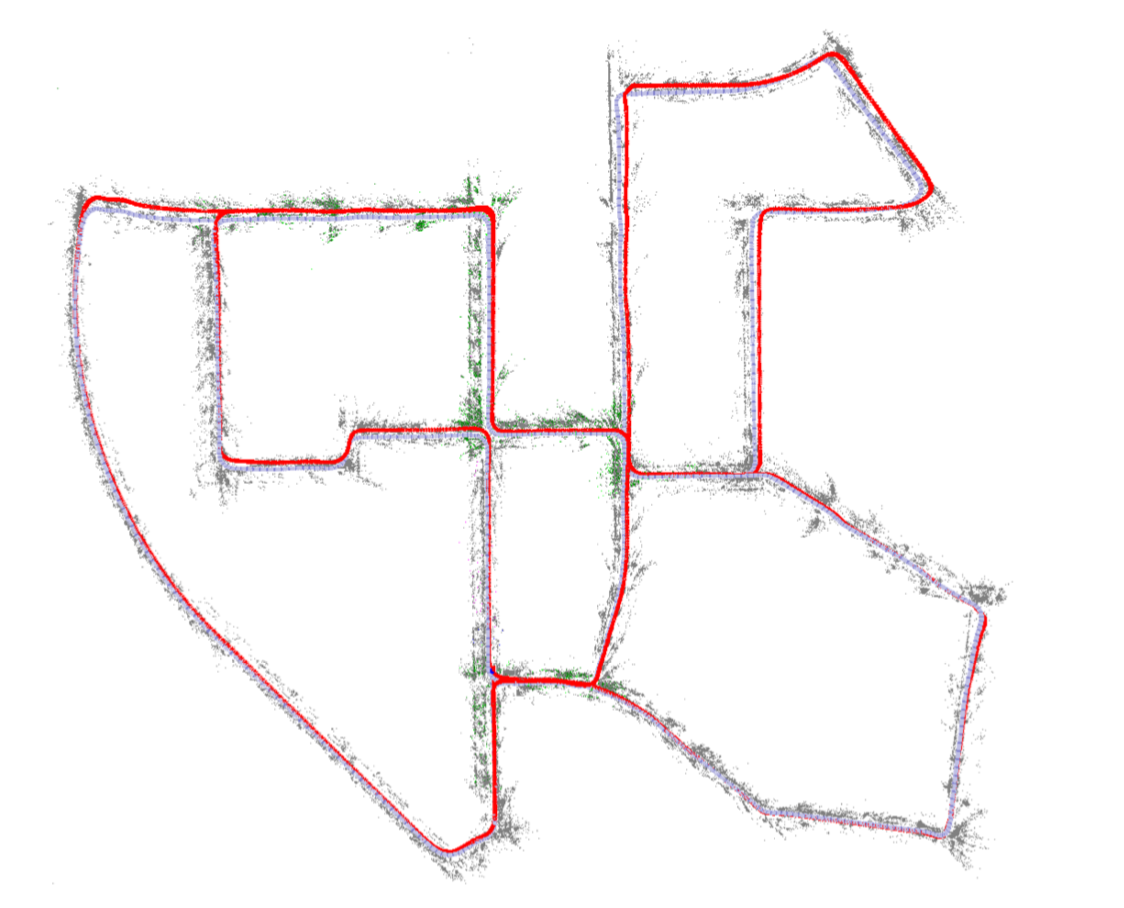
\includegraphics[width=1\textwidth]{slam8}
    \column{.3\textwidth}
    \begin{itemize}
    \item \textbf{S}imultaneous
    \item \textbf{L}ocalization
    \item \textbf{A}nd
    \item \textbf{M}apping
    \end{itemize}  
  \end{columns}
\end{frame}

\subsection{Related work}
\subsubsection*{History}
\begin{frame}
  \frametitle{History:   LSD SLAM}
  \begin{columns}
    \column{.7\textwidth}
    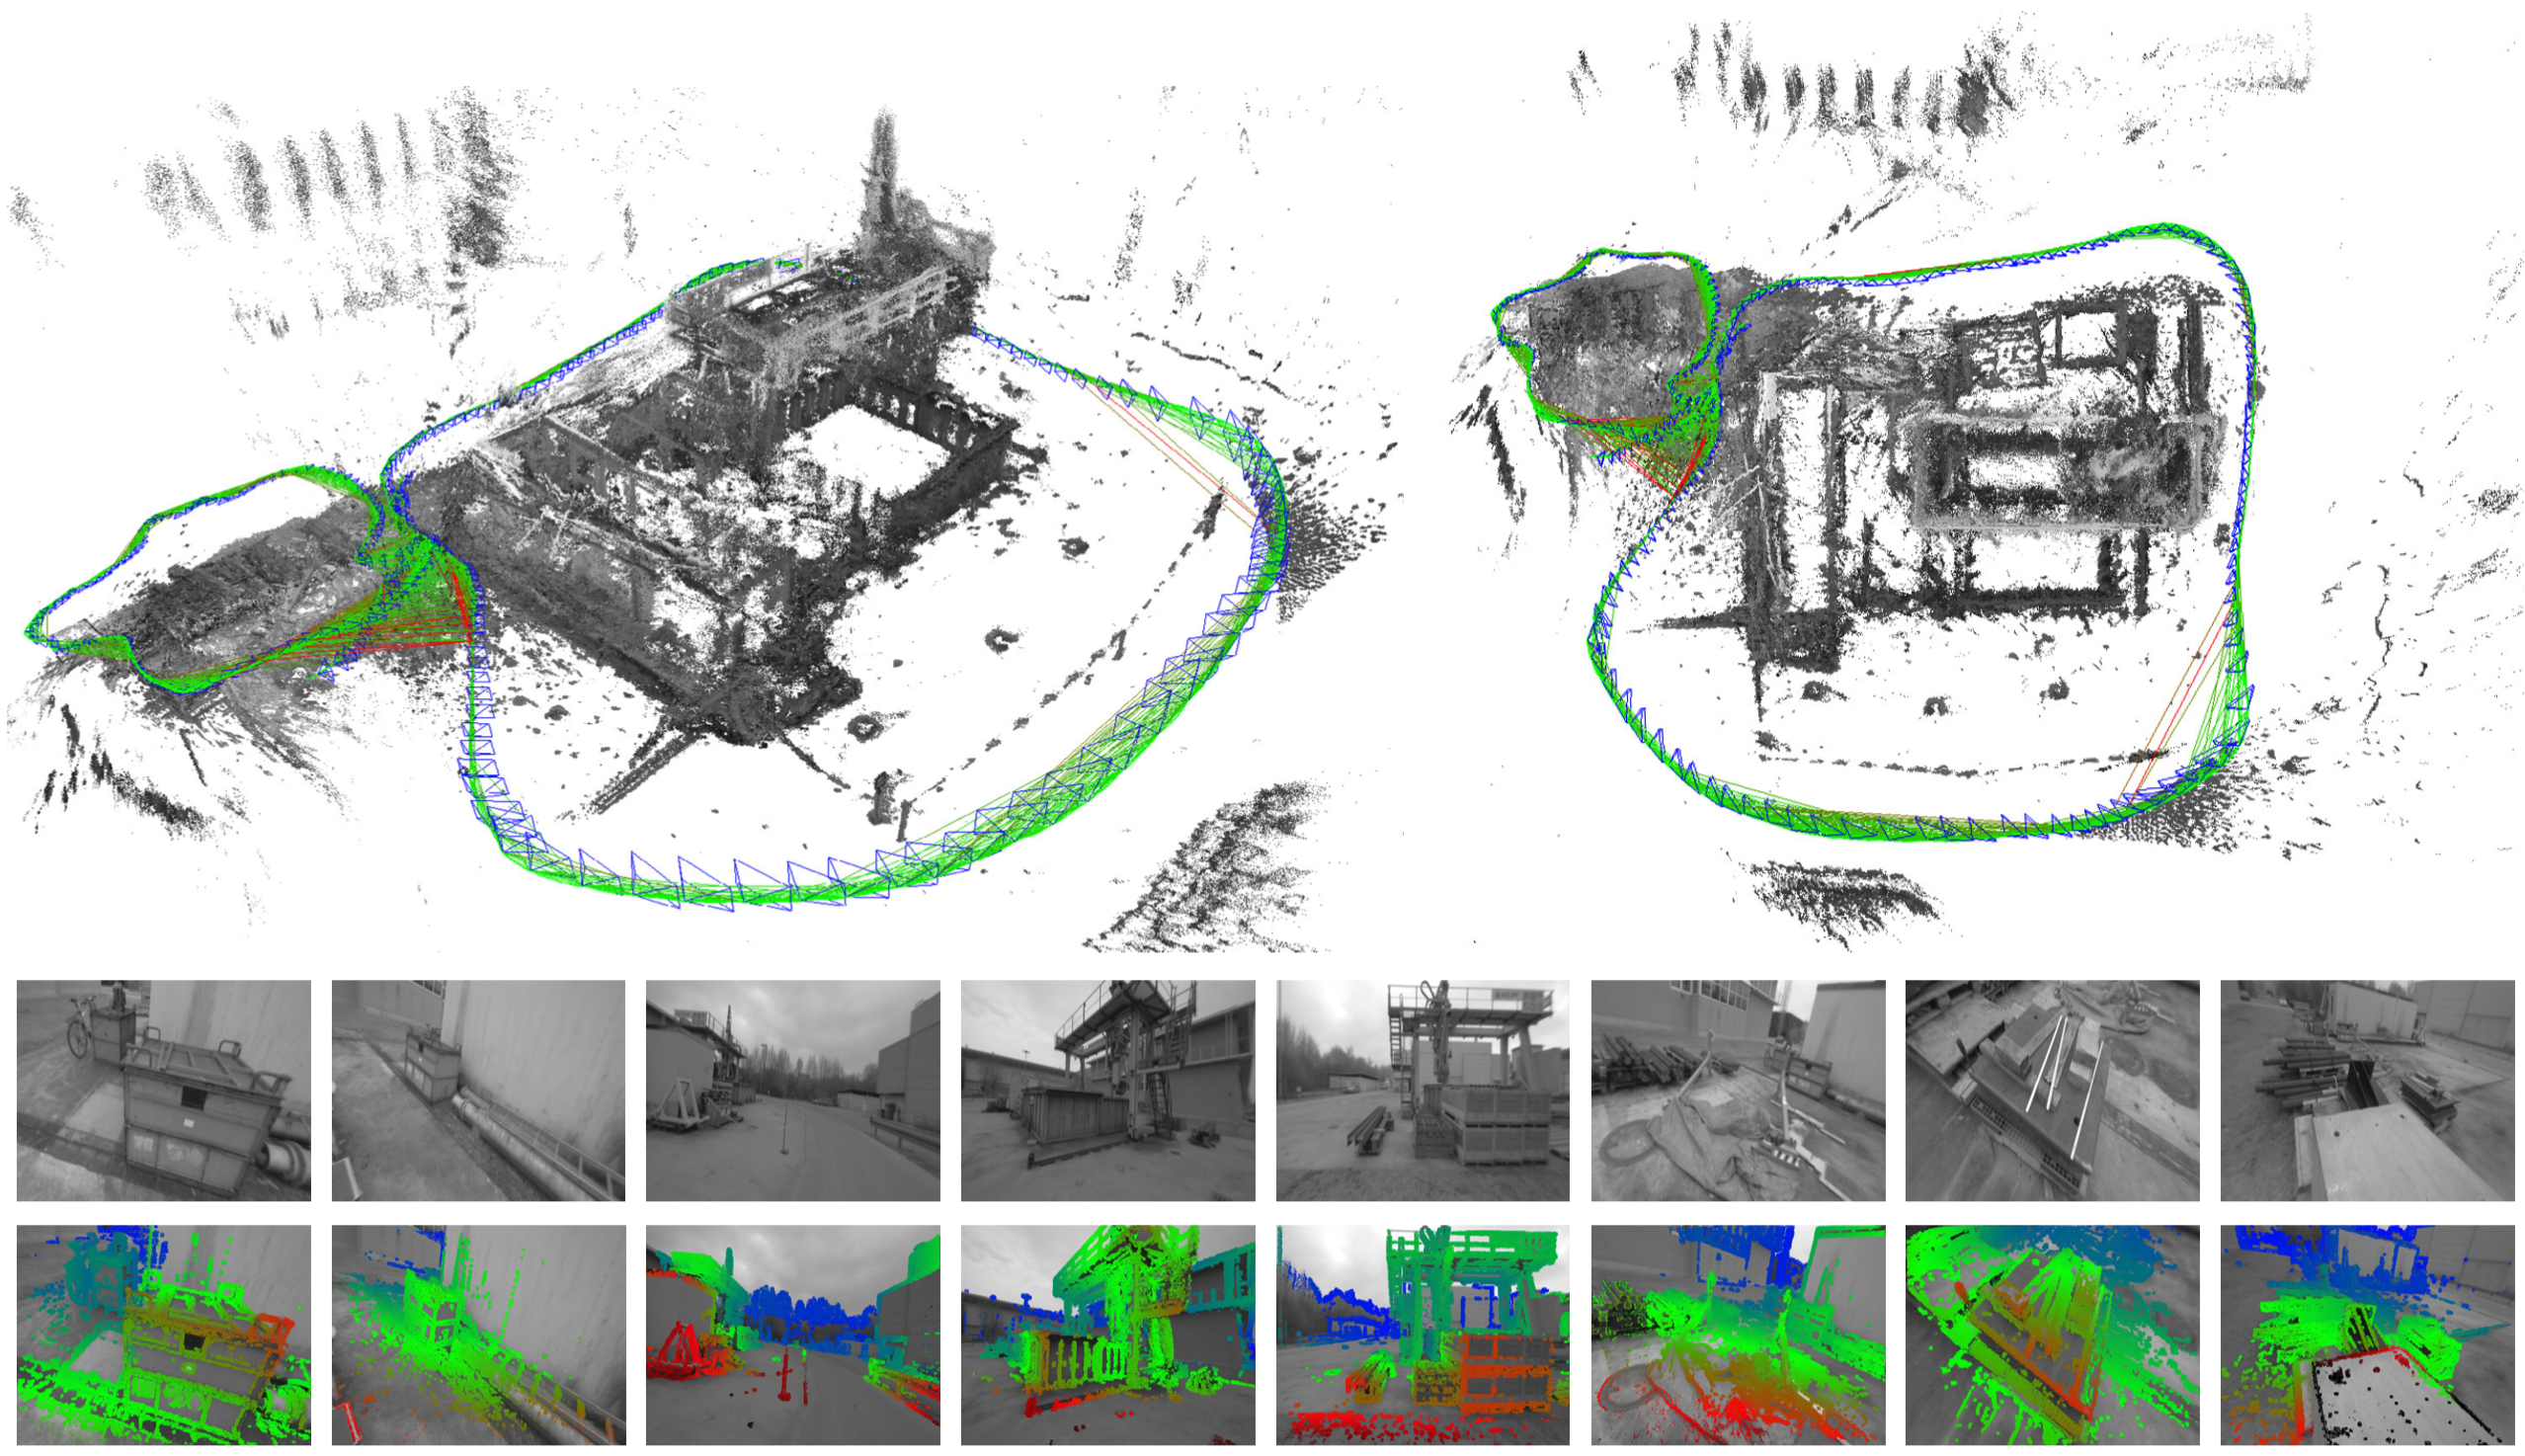
\includegraphics[width=1\textwidth]{lsdSlam1}
    \includegraphics[width=1\textwidth]{lsdSlam2}
    \column{.3\textwidth}
    \textbf{L}arge-\textbf{S}cale \textbf{D}irect \textbf{SLAM}:\\\medskip
    \begin{block}{\textbf{Age:}}
      \textsl{2014}
    \end{block}
    \bigskip
    \begin{block}{\textbf{Matching:}}
      feature-\textsl{less}
    \end{block}
    \bigskip
    \begin{block}{\textbf{Cameras:}}
      monocular
    \end{block}
  \end{columns}
\end{frame}
\subsubsection*{State of the art}
\begin{frame}
  \frametitle{State of the art:   ORB SLAM 2 }
  
  \includegraphics[width=1\textwidth]{orb2slam}
  \medskip
  \textbf{ ORB SLAM 2}:
  \smallskip
  \begin{columns}
    \column{.23\textwidth}
    \begin{block}{\textbf{Age}}
      June\\
      \textsl{2017}
    \end{block}
    \column{.43\textwidth}
    \begin{block}{\textbf{Matching:}}
      \textbf{stereo} keypoints\\
      bundle \textbf{adjustment}
    \end{block}
    \column{.33\textwidth}
    \begin{block}{\textbf{Cameras:}}
      monocular\\
      stereo\\
      \textbf{RGB-D}
    \end{block}
 
  \end{columns}
\end{frame}

\subsection{Problem}
\begin{frame}
  \frametitle{Problem: Other SLAM approaches }
  \begin{columns}
    \column{.4\textwidth}
    \textbf{Issues:}
    \begin{itemize}
    \item Computationally \textbf{Heavy}
      \bigskip
    \item High Theoretical \textbf{Complex}ity
      \bigskip
    \item \textbf{How} to implement it in practice ?
    \end{itemize}
    \column{.6\textwidth}
    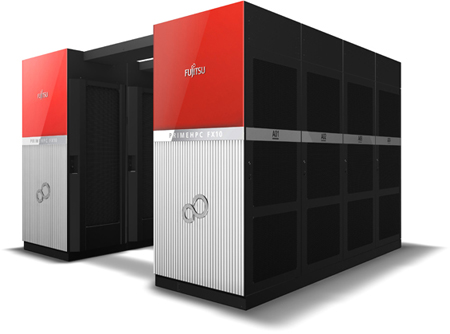
\includegraphics[width=.6\textwidth]{superPc}
    \smallskip
    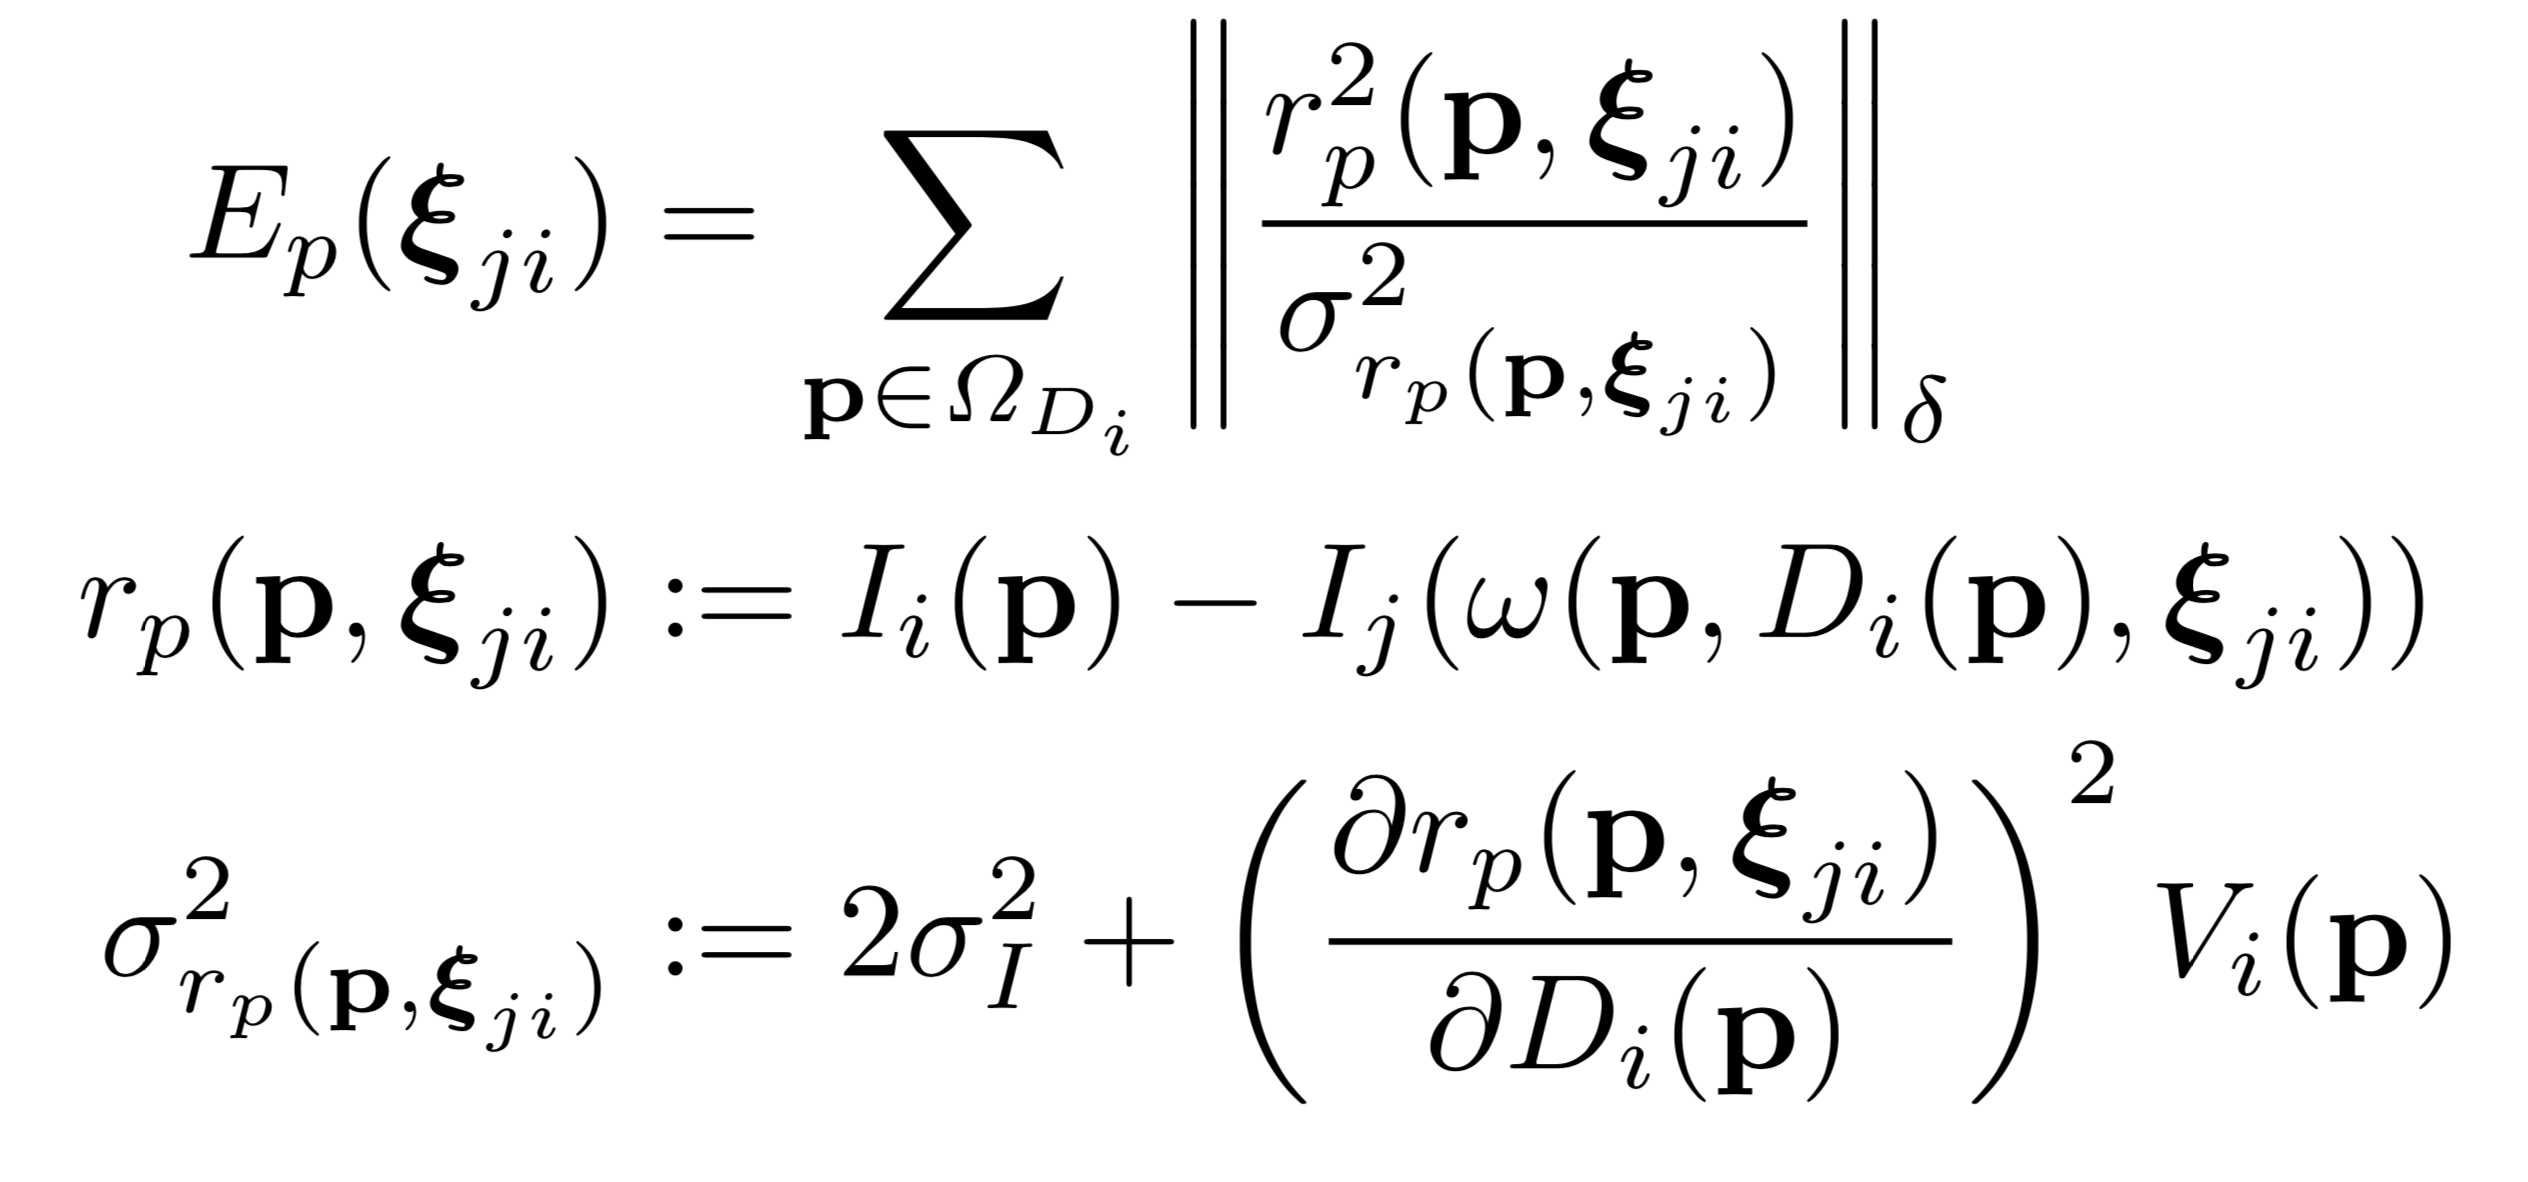
\includegraphics[width=1\textwidth]{lsdComplex}
  \end{columns}
\end{frame}


\subsection{Proposed solution}
\begin{frame}
  \frametitle{ProSLAM:    Proposed solution}

  \centering
  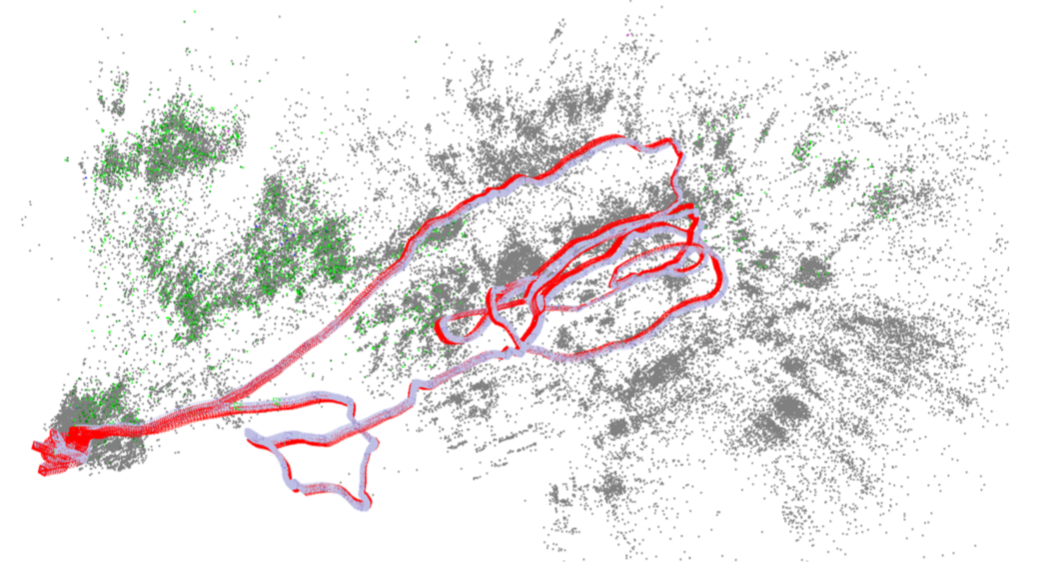
\includegraphics[width=1\textwidth]{slam7}
  \begin{columns}
    \column{.23\textwidth}
    \begin{block}{\textbf{Age}}
      September\\
      \textsl{2017}
    \end{block}
    \column{.53\textwidth}
    \begin{block}{\textbf{Matching:}}
      feature-based:\quad\textbf{landmarks}\\
      \textbf{local} bundle adjustment
    \end{block}
    \column{.23\textwidth}
    \begin{block}{\textbf{Cameras:}}
      stereo
    \end{block}
 
  \end{columns}

\end{frame}
 
\section{ Algorithm}
\subsection*{ProSLAM}
\begin{frame}
  \frametitle{ProSLAM: From above }
  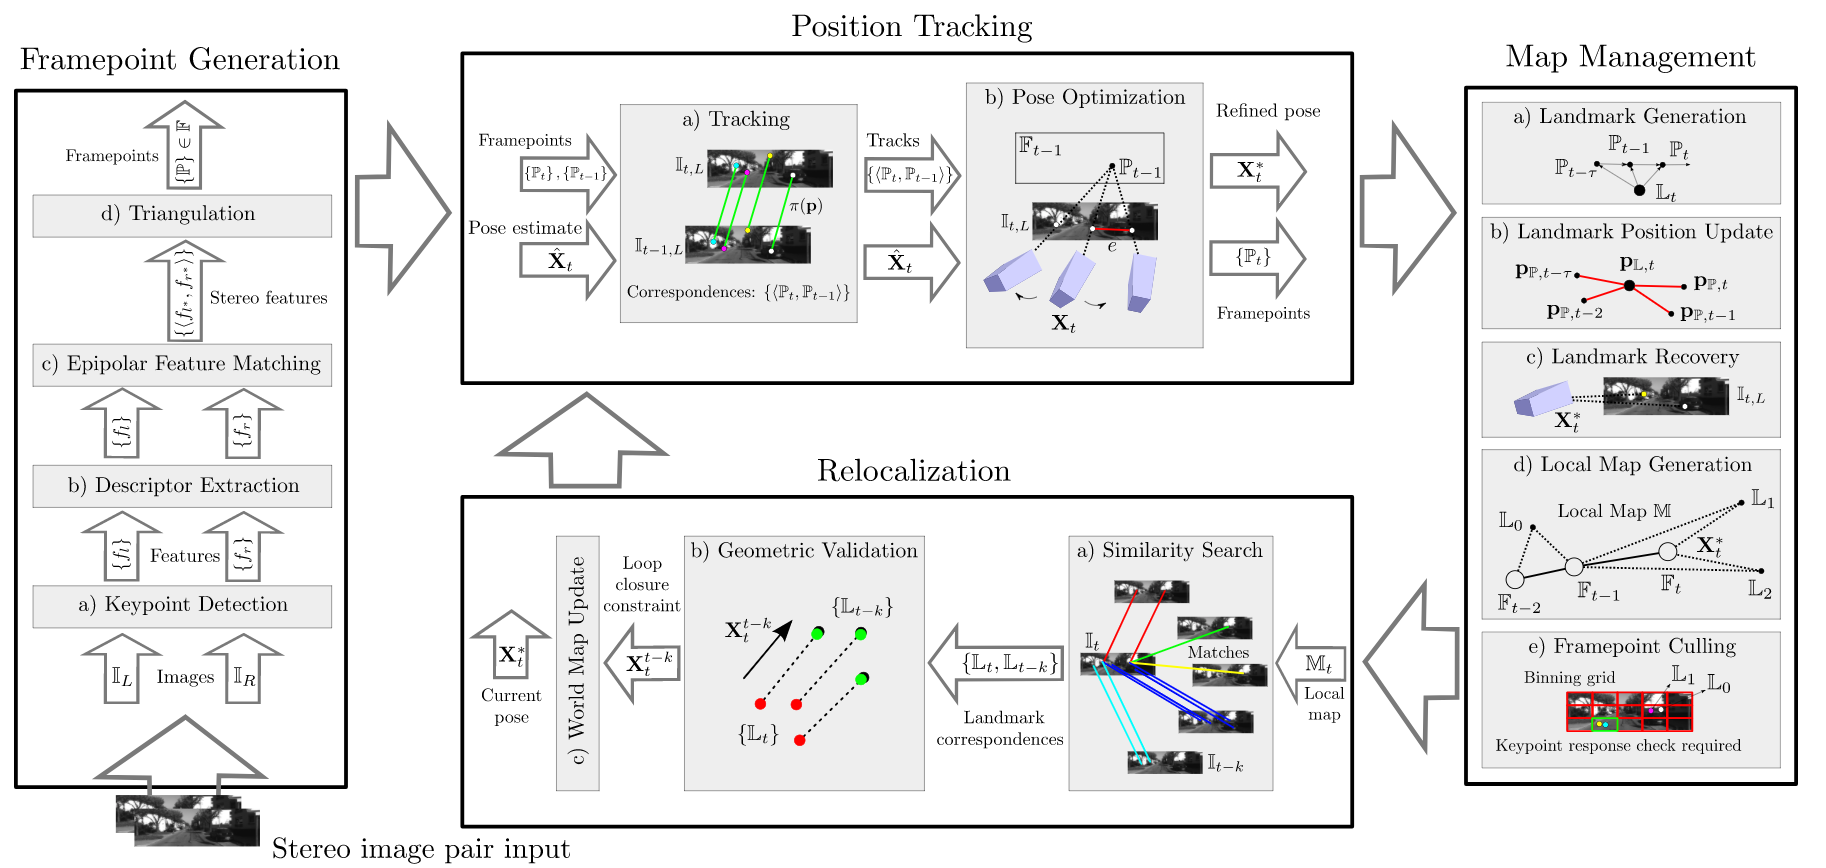
\includegraphics[width=1\textwidth]{slam0}
\end{frame}

\subsection{Data Structs}
\begin{frame}
  \frametitle{Data Structs: visual representation }
  \centering
  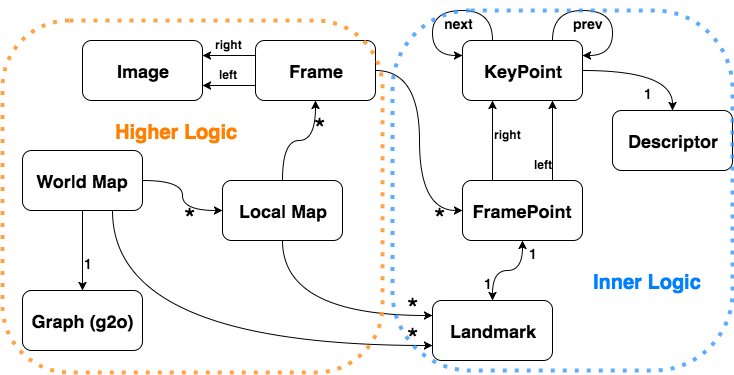
\includegraphics[width=.7\textwidth]{dataStructs}
  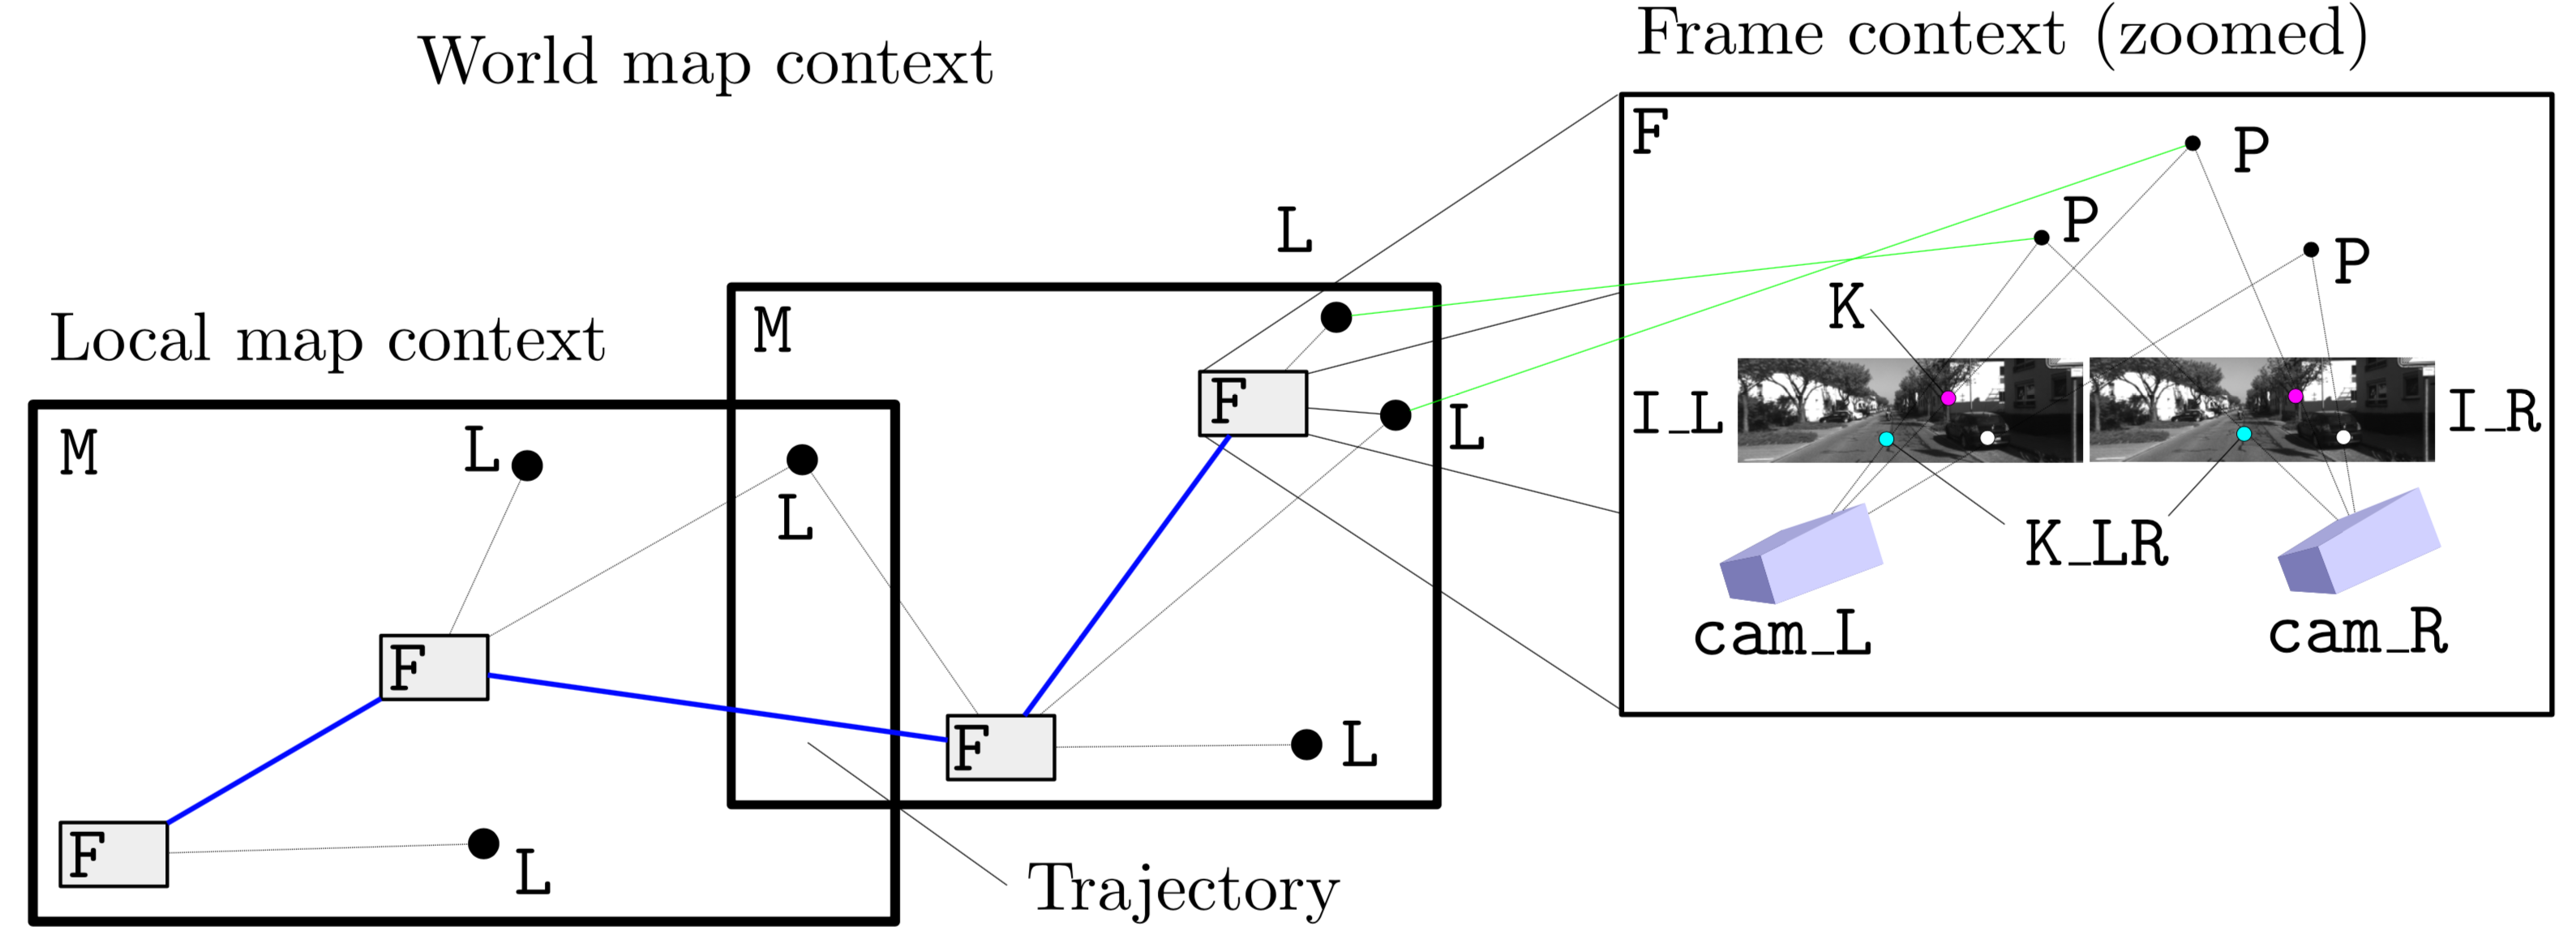
\includegraphics[width=.7\textwidth]{HDslam5}
\end{frame}

\subsection{Pipeline}
\begin{frame}
  \frametitle{Pipeline: four  phases}
  \centering
  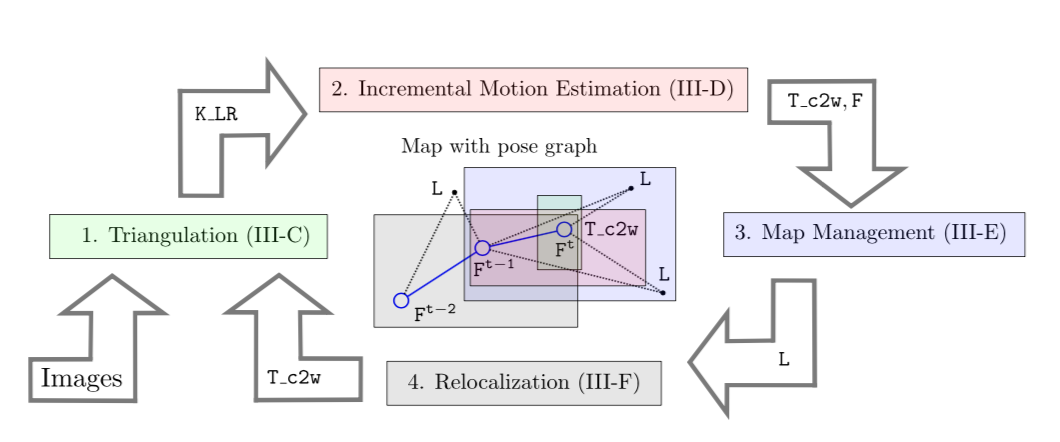
\includegraphics[width=.8\textwidth]{slam6}
  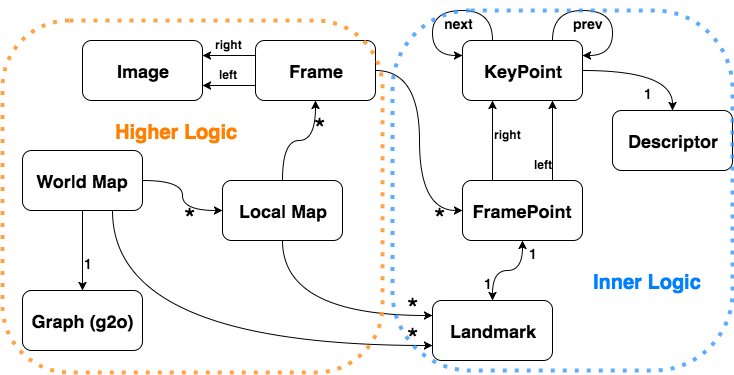
\includegraphics[width=.7\textwidth]{dataStructs}
\end{frame}



\subsubsection*{Triangulation}
\begin{frame}
\frametitle{Triangulation: phase one}
  \begin{figure}
    \centering
    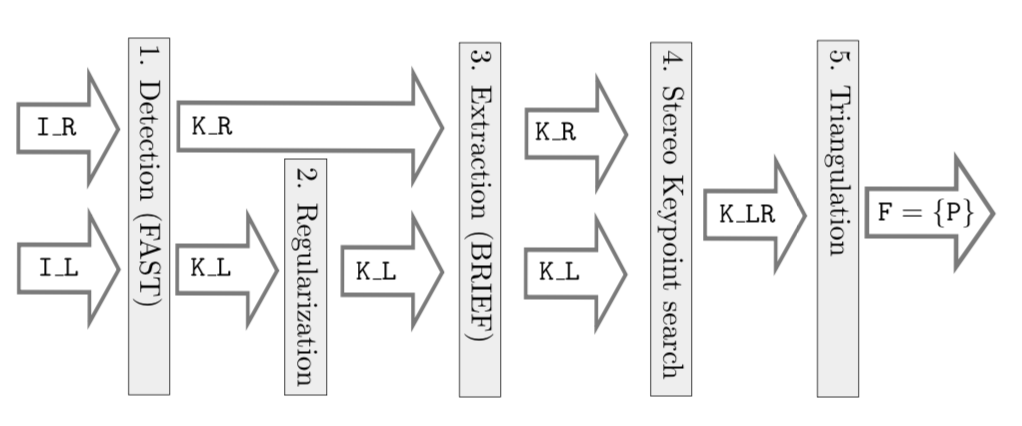
\includegraphics[width=.8\textwidth]{slam4}
  \end{figure}
  \textbf{Framepoint} coords:
  \begin{columns}
    \column{.5\textwidth}
    \begin{equation}
      p_z = \frac{\overbrace{B}^{\text{stereo camera baseline}}}{K_r.c - K_l.c}
    \end{equation}
    \column{.5\textwidth}
    \begin{equation}
      p_x = \frac{p_z}{\underbrace{F_x}}K_l.c - C_x
    \end{equation}
    \begin{equation}
      p_y = \frac{p_z}{\underbrace{F_y}_{\text{focal length}}}K_l.r - C_y
    \end{equation}
  \end{columns}
\end{frame}

\begin{frame}
  \frametitle{Triangulation : Intuition}
\begin{figure}
    \centering
    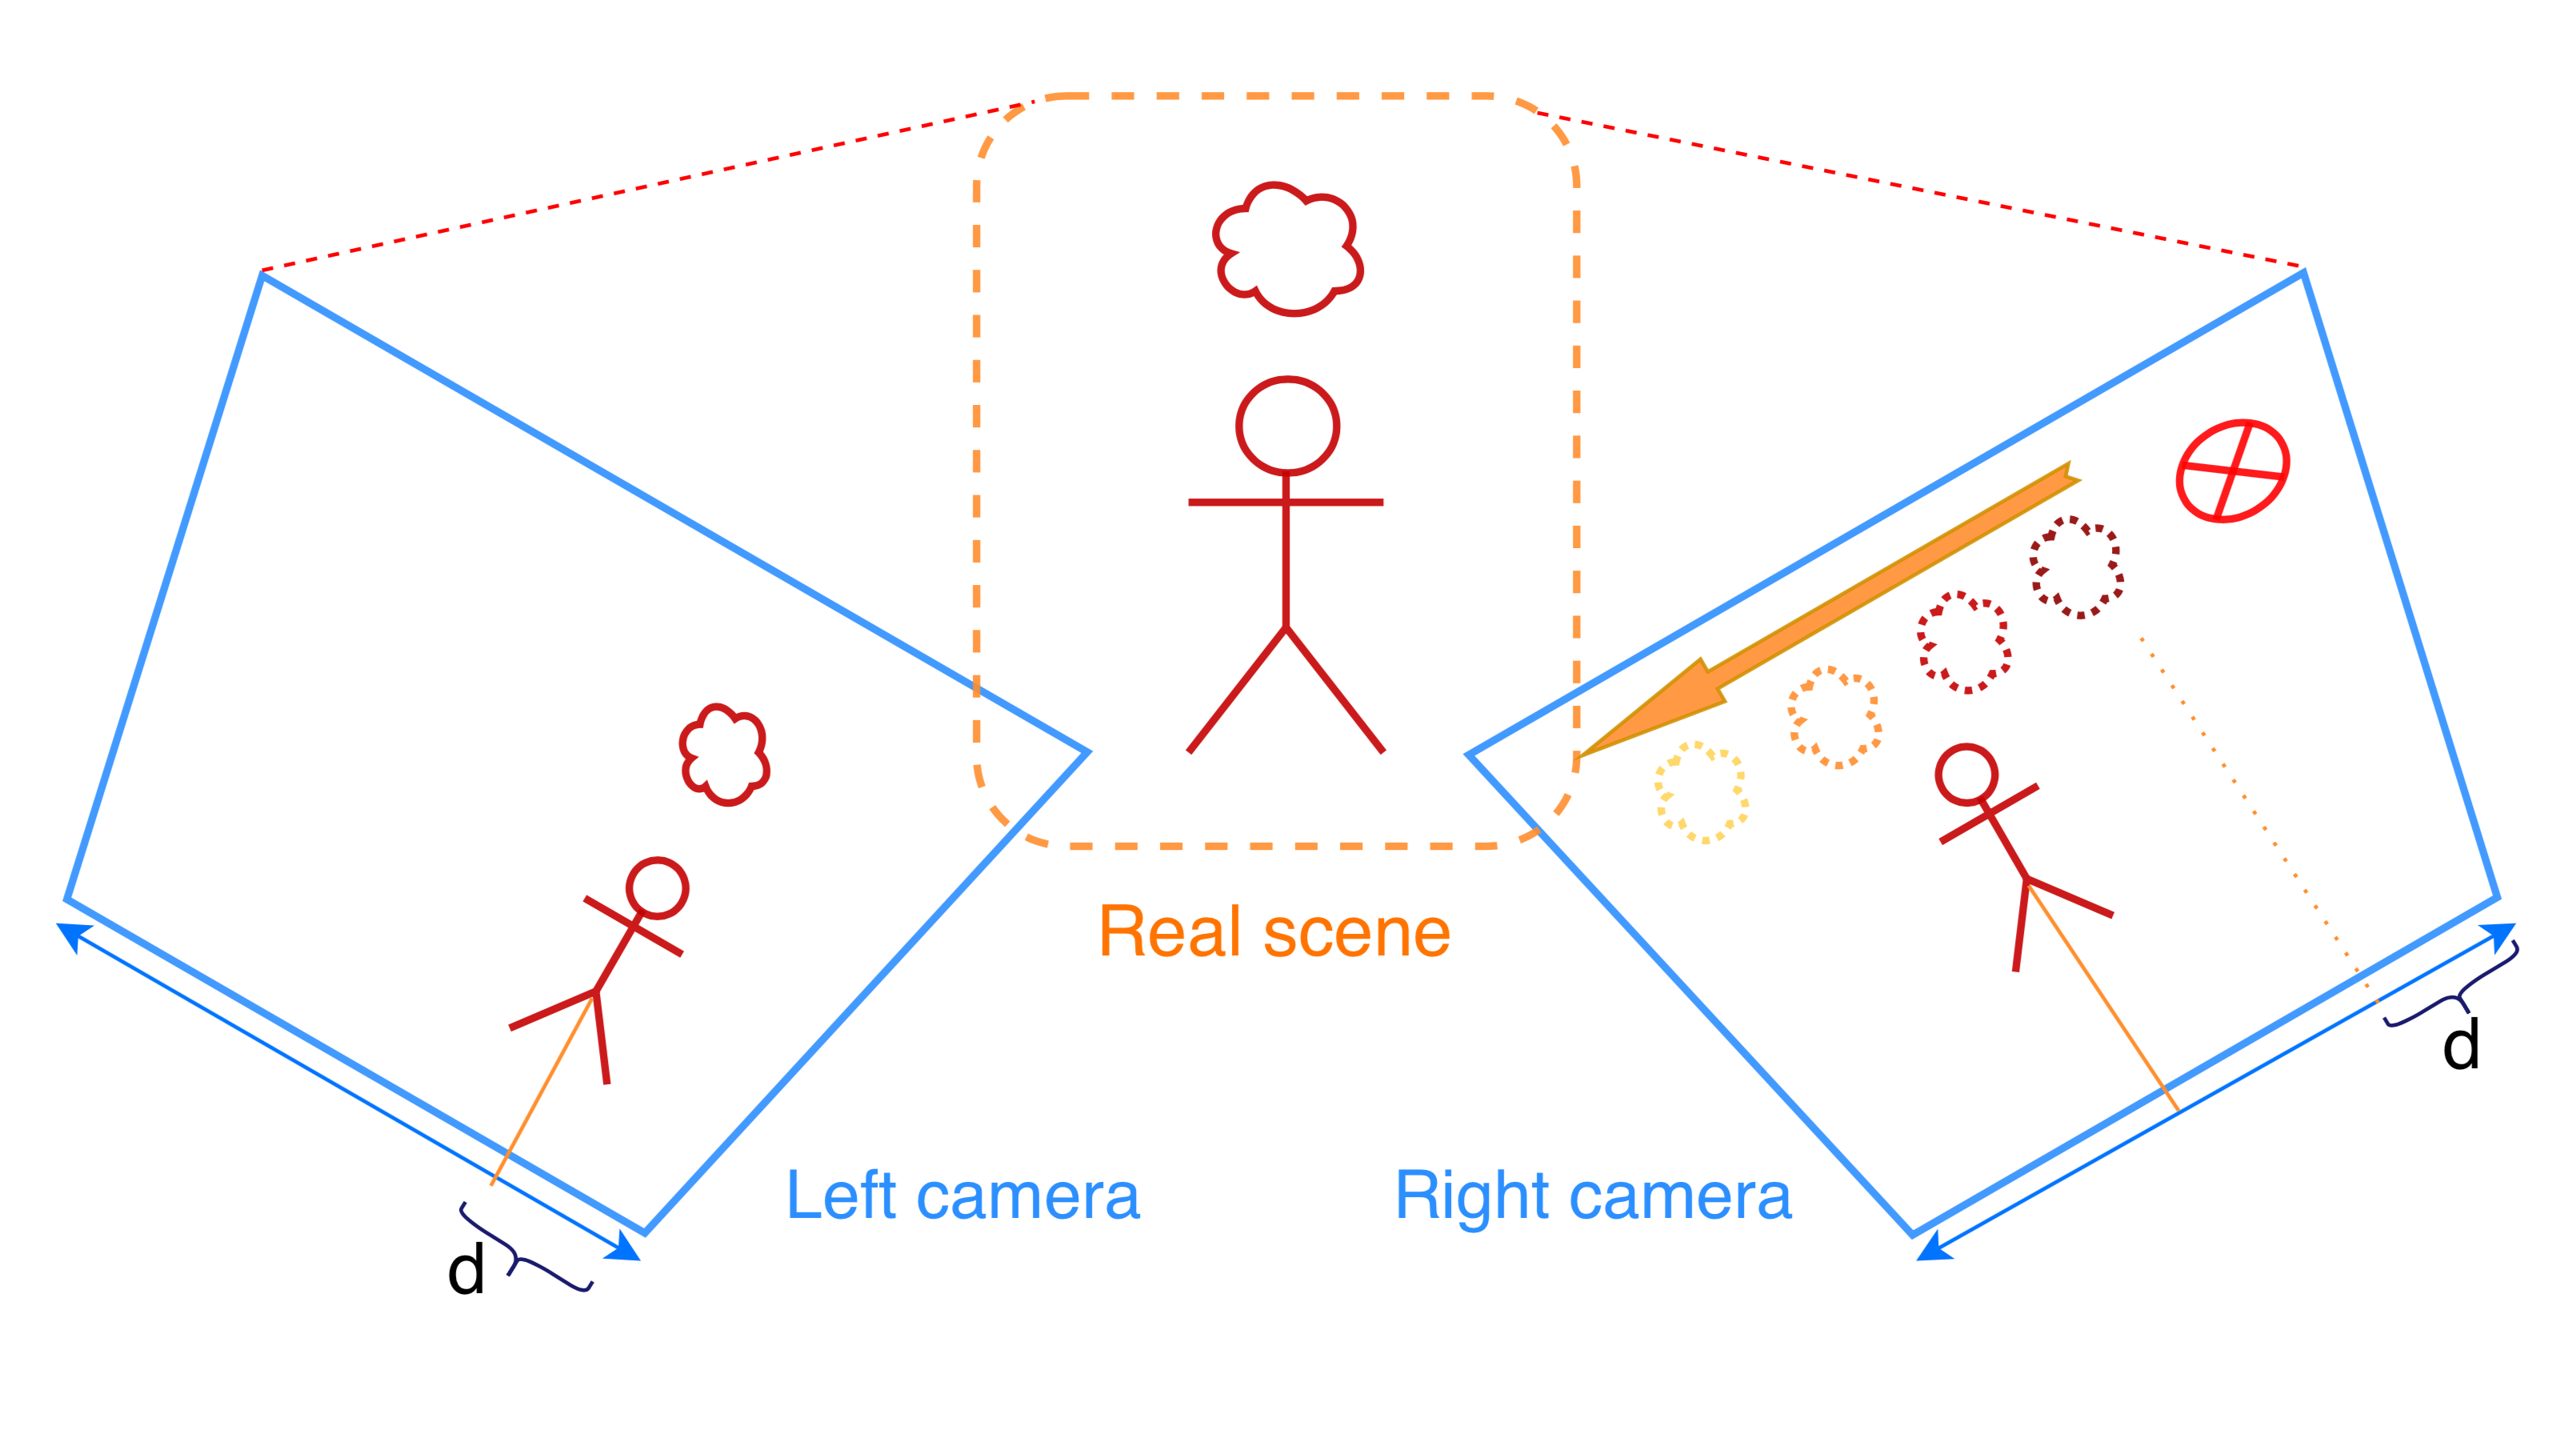
\includegraphics[width=.9\textwidth]{triangIntu}
  \end{figure}
  \begin{block}{\textbf{Correspondence} matching:}
    \begin{itemize}
      \item{Expected on the \textbf{left side} of the other image.}
      \item{Candidates \textbf{sorted} with euclidean distance metric.}
      \end{itemize}
  \end{block}
\end{frame}


\subsubsection*{Incremental Motion Estimation}
\begin{frame}
  \frametitle{Incremental Motion Estimation: phase two}

  \begin{figure}
    \centering
    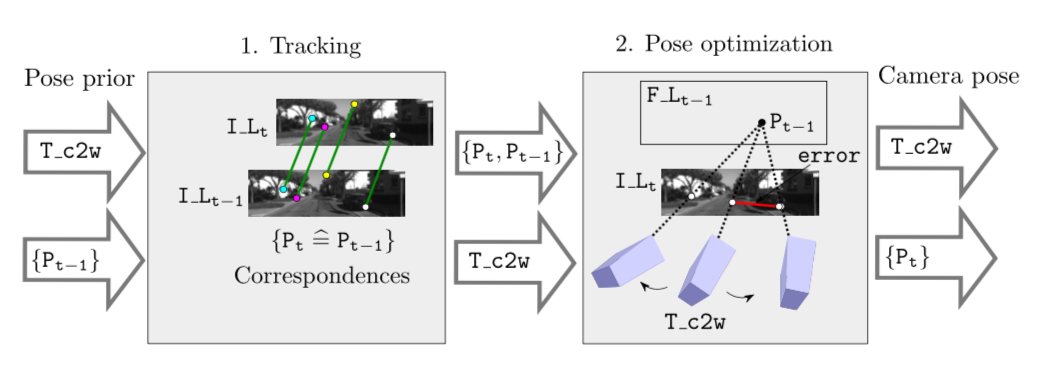
\includegraphics[width=.8\textwidth]{slam2}
  \end{figure}
  \begin{equation}
    \overbrace{K_P}^{\text{new keypoint}} = \pi( P_L* \underbrace{T_{w2c}*\overbrace{P_{t-1}}^{\text{framepoint}}.p_w }_{P_{t-1}.p_c})
  \end{equation}
  \begin{center}
  $\pi$: cam proj function, $P_{L}$: left cam proj matrix, $T_m$: motion
  \end{center}
  \begin{block}{\textbf{Constant} velocity evolution model:}
    \begin{equation}
      T_m = F_{t-1}.T_{w2c}*F_{t-2}.(T_{w2c})^{-1}
    \end{equation}
    \begin{equation}
      T_{w2c} = T_m* F_{t-1}.T_{w2c}
    \end{equation}
  \end{block}
\end{frame}


\subsubsection*{Map Management}
\begin{frame}
  \frametitle{Map Management: phase three}
 \begin{figure}
    \centering
    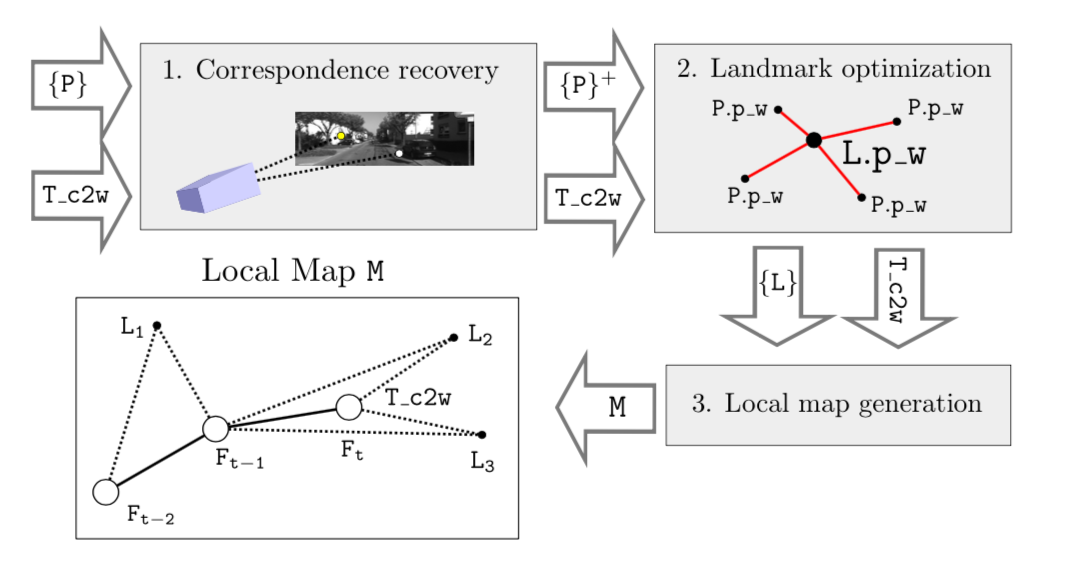
\includegraphics[width=.8\textwidth]{slam3}
  \end{figure}
  \begin{columns}
    \column{.28\textwidth}
    \begin{block}{Correspondence recovery}
      Bookkeping unmatched framepoints
    \end{block}
    \column{.34\textwidth}
    \begin{block}{Landmark optimization}
      Refine extimation with information filter
    \end{block}
    \column{.38\textwidth}
    \begin{block}{Local map generation}
      If translation or rotation wtr previous one exceeds threshold    
    \end{block}
  \end{columns}
\end{frame}


\subsubsection*{Relocation}
\begin{frame}
  \frametitle{Relocation: phase four}
  \begin{figure}
    \centering
    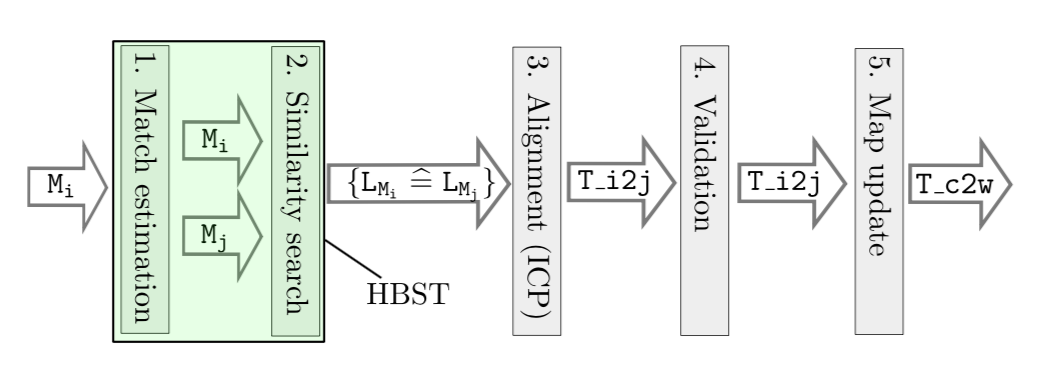
\includegraphics[width=.8\textwidth]{slam1}
  \end{figure}
  \begin{equation}
    M_i \xrightarrow[\text{relocalize}]{} M_j \qquad j: 1, \dots, i-1
  \end{equation}
  \smallskip
  \begin{itemize}
  \item{Compute relative transformations $T_{i2j}$.}
  \item{Validate through \textbf{outliers} and \textbf{avg error}.}
  \end{itemize}
\end{frame}

\section{ Results }
\begin{frame}
  \frametitle{Results:   Translational and rotational Errors}
  % translational error   rotational error
  \begin{columns}
    \column{.5\textwidth}
    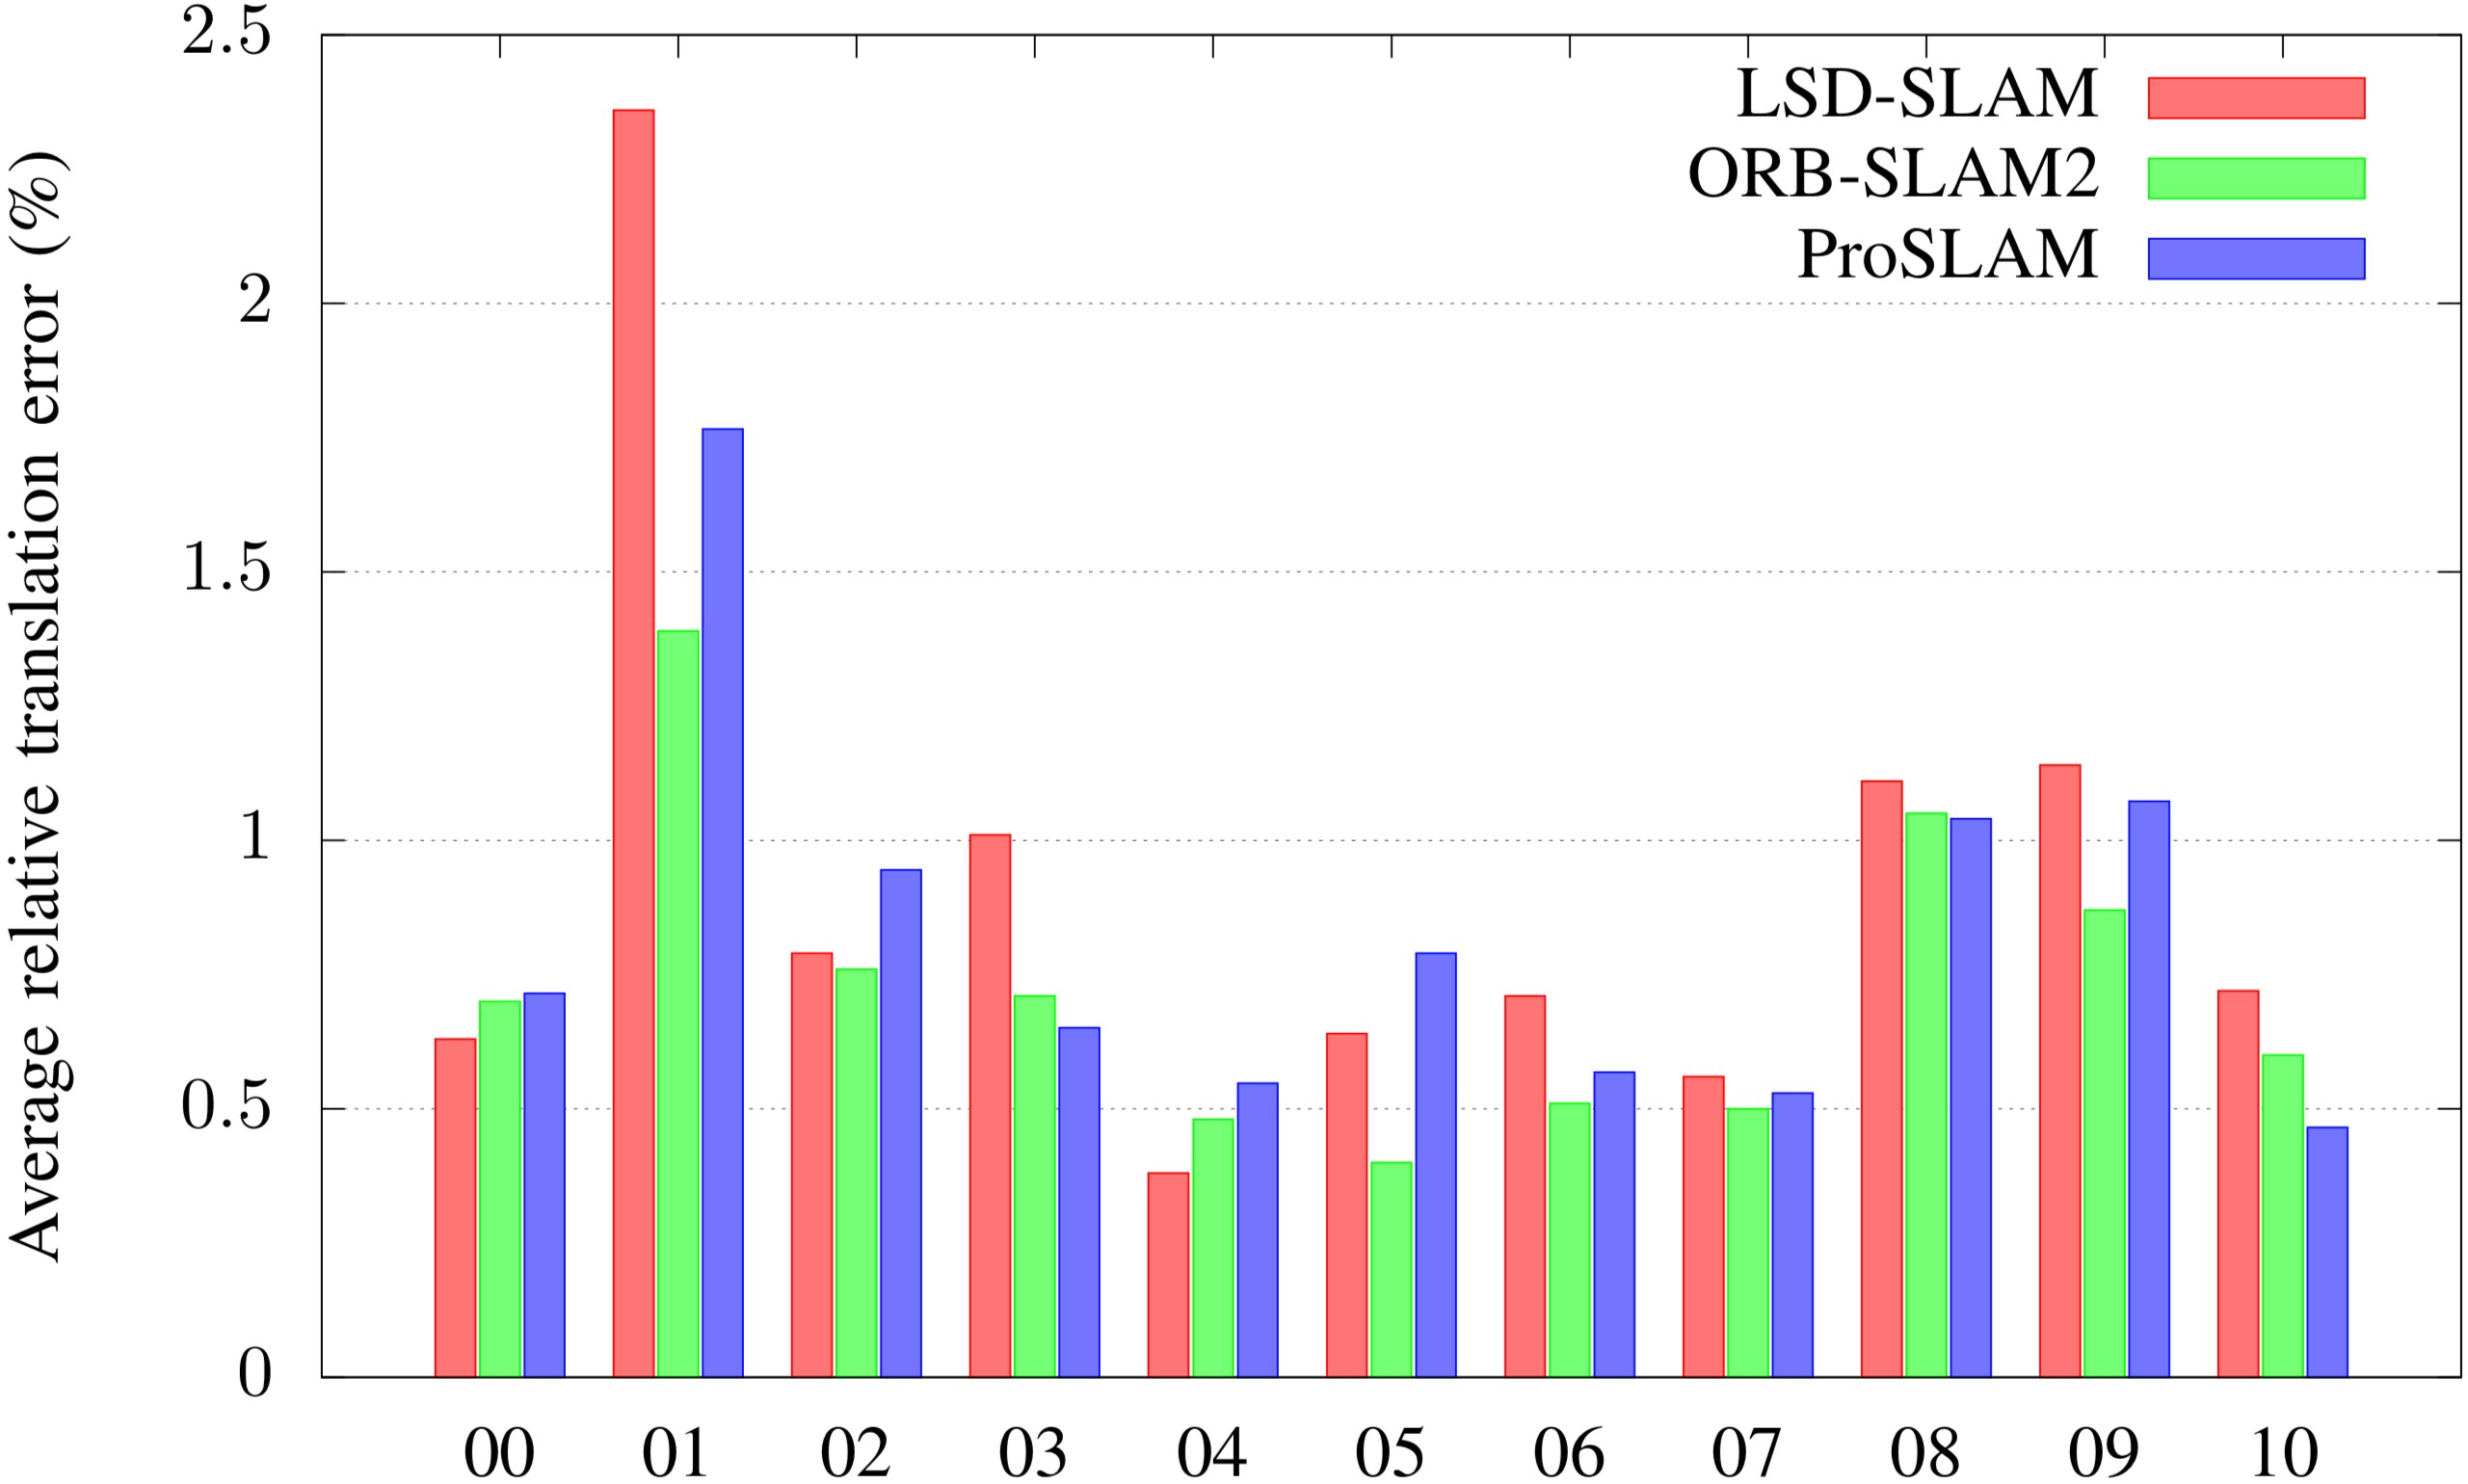
\includegraphics[width=1\textwidth]{HDslam9}
    \column{.5\textwidth}
    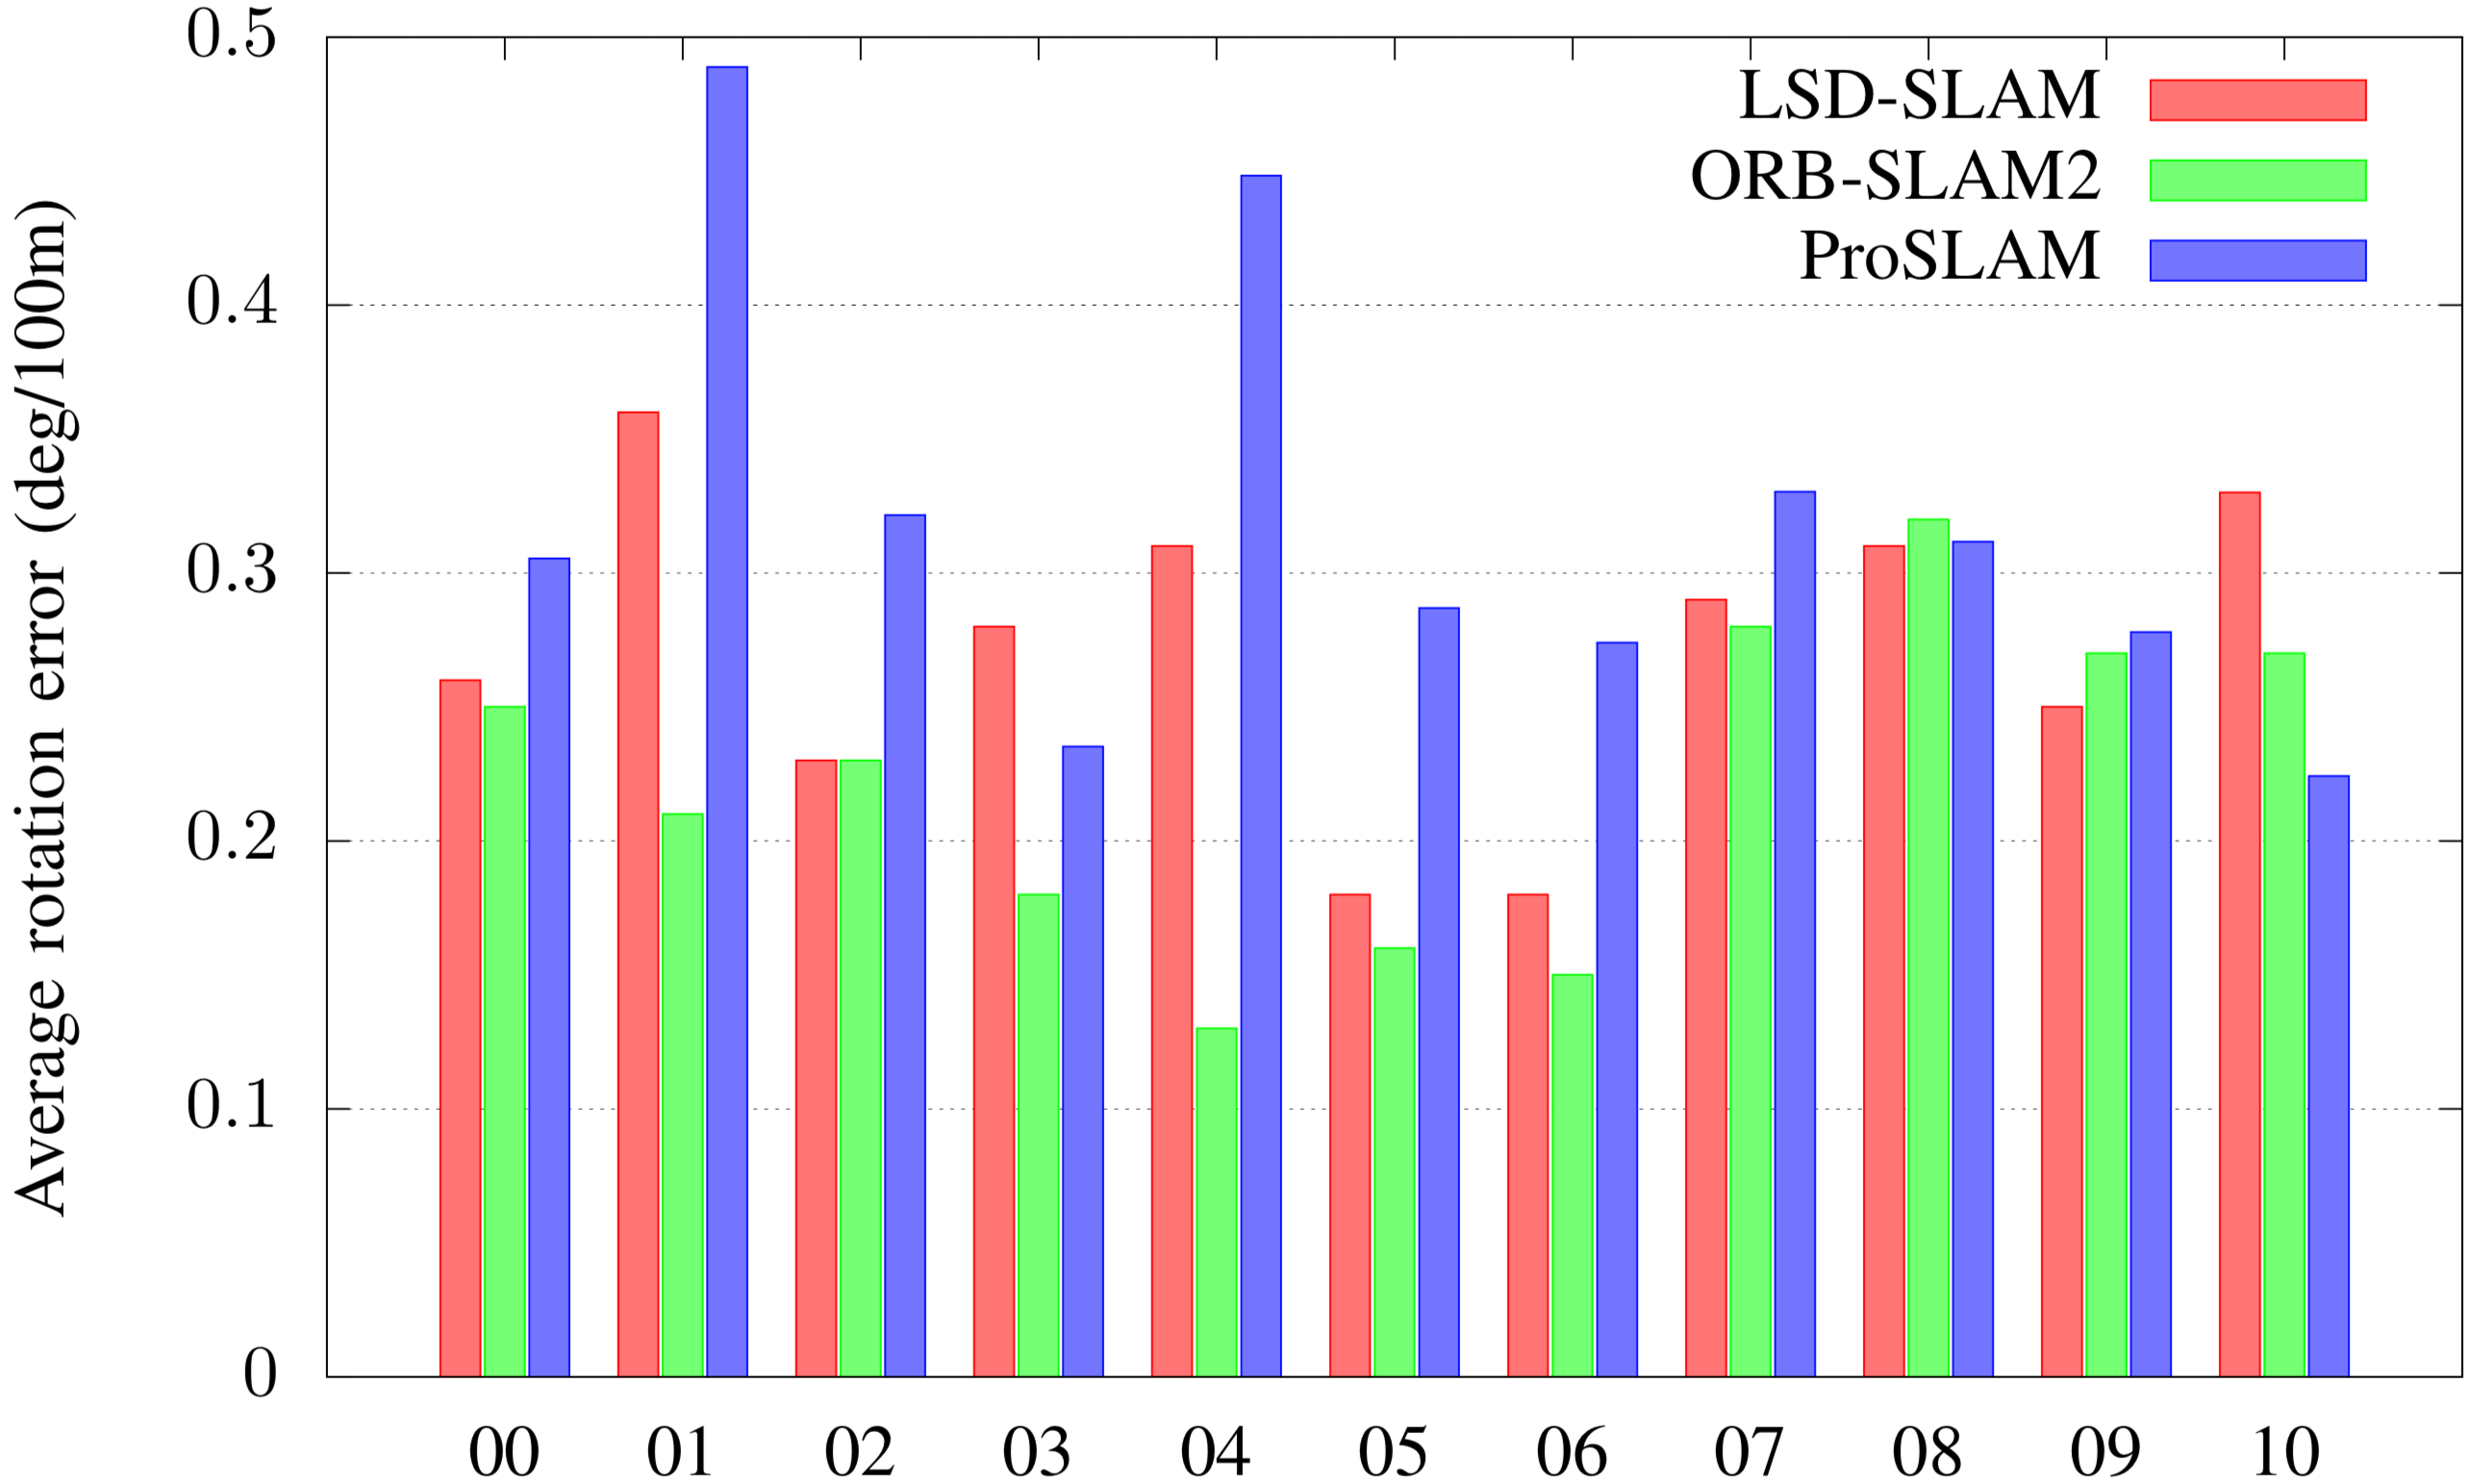
\includegraphics[width=1\textwidth]{HDslam10}
  \end{columns}

  \begin{block}{\centering\textbf{Positive:}}
    Same \textbf{translational} error as state of the art.
  \end{block}
  \begin{block}{\centering\textbf{Negative:}}
    Losing in \textbf{rotational} error evaluations.
  \end{block}
\end{frame}

\section{ Conclusion}
\begin{frame}
  \frametitle{Conclusion}
  \textbf{ To summarize: }
  \begin{itemize}
  \item Results shown \textbf{nearly} state of the art performance.
  \item Algorithm runs on portable computer in real time (\textsl{light-weight}).
  \item Open source and \textbf{understable} implementation for newcomers.
  \end{itemize}
  \begin{block}{ Take home message}
    If you want to learn SLAM, \textbf{ProSLAM} is the way to start with.
  \end{block}
\end{frame}

\begin{frame}
  \frametitle{Demo video}
  \begin{center}
  Placeholder for the movie
   % \movie[height = 0.72\textwidth, width = 0.72\textwidth]{}{./vidSlam.mov}
  \end{center}
\end{frame}

\begin{frame}
  \frametitle{That's all}
  \begin{center}
    \textsl{Thank you for your attention !}\\\bigskip
    \textsl{Any \textbf{question} ?}\\\bigskip
    \textsl{Feel free to ask !}
  \end{center}
\end{frame}


\end{document}
